\documentclass[a4paper,12pt,twocolumn]{article}

% Packages
\usepackage{graphicx}
\usepackage{caption} % more customisation options for captions, used for fontsize in figures.
\usepackage{amsmath} % more function within maths environments, namely \text{}

% Making cites superscript
\usepackage[sorting=none]{biblatex}
\DeclareCiteCommand{\supercite}[\mkbibsuperscript]
{\iffieldundef{prenote}
	{}
	{\BibliographyWarning{Ignoring prenote argument}}%
	\iffieldundef{postnote}
	{}
	{\BibliographyWarning{Ignoring postnote argument}}}
{\usebibmacro{citeindex}%
	\bibopenbracket\usebibmacro{cite}\bibclosebracket}
{\supercitedelim}
{}
\let\cite=\supercite

% Adding the bibliography file
\addbibresource{references.bib}

\begin{document}
	
	\begin{titlepage}
		\begin{center}
			
			\thispagestyle{empty}
			
			\Huge{
				\textbf{UCD School Of Physics}
			}
			
			\vspace{1cm}	
			
			
\includegraphics[scale=0.08]{UCDLogo.png}
			
			\vspace{1cm}
			
			\large{
				\textbf{PHYC30170 Physics with Astronomy and Space Science Lab 1; \\
					CCDs and Spectroscopy \\
					\vspace{1cm}
					18/10/2022 \\
					\vspace{1cm}
					Daragh Hollman}
			} \\
			
		\end{center}
	\end{titlepage}
	
	\twocolumn[
	\begin{@twocolumnfalse}
		\begin{abstract}
			The aim of this experiment was to calibrate a CCD for spectroscopy and determine the resolution of a spectrograph. This was done by comparing the emission spectrum of a mercury arc lap to reference values... INSERT RESULTS.
		\end{abstract}
	\end{@twocolumnfalse}
	]
	
	\section{Introduction}
	
	\section{Theory}
		\subsection{Diffraction}
			A diffraction grating is used to split incident light into its separate wavelengths. As a diffraction grating is an array of very narrow and evenly spaced slits, the diffraction pattern from each slit interferes such that the light disperses by a angle $\theta$ as described by equation \ref{eq:diffraction}\cite{universityPhysics}.
			\begin{equation}
				n \lambda = d sin\theta
				\label{eq:diffraction}
			\end{equation} where $d$ is the spacing between the slits, 	$\lambda$ is the wavelength of the incident light, $\theta$ is the angle which the light is diffracted by and $n$ is a positive integer. This process is the primary element of a spectrograph.\\
		
		\subsection{The Spectrograph}	
			A spectrograph is an instrument used to measure incoming light and record its spectrum\cite{atnf}. It splits the incoming light based on its wavelength through diffraction. There are five key components to a spectrograph: telescope, slit, collimator, diffraction grating and detector, as shown in figure \ref{fig:spectrograph}. The telescope focuses the incident light on the slit which only allows a small (ideally 1D) slice of the target through\cite{manual}. The light diverges after the slit and so a collimator is used to make the rays parallel again to ensure that all parts of the light hit the grating at the same angle of incidence. The light then hits the grating and is diffracted at an angle according to its wavelength which the detector picks up.
		
			\begin{figure}
				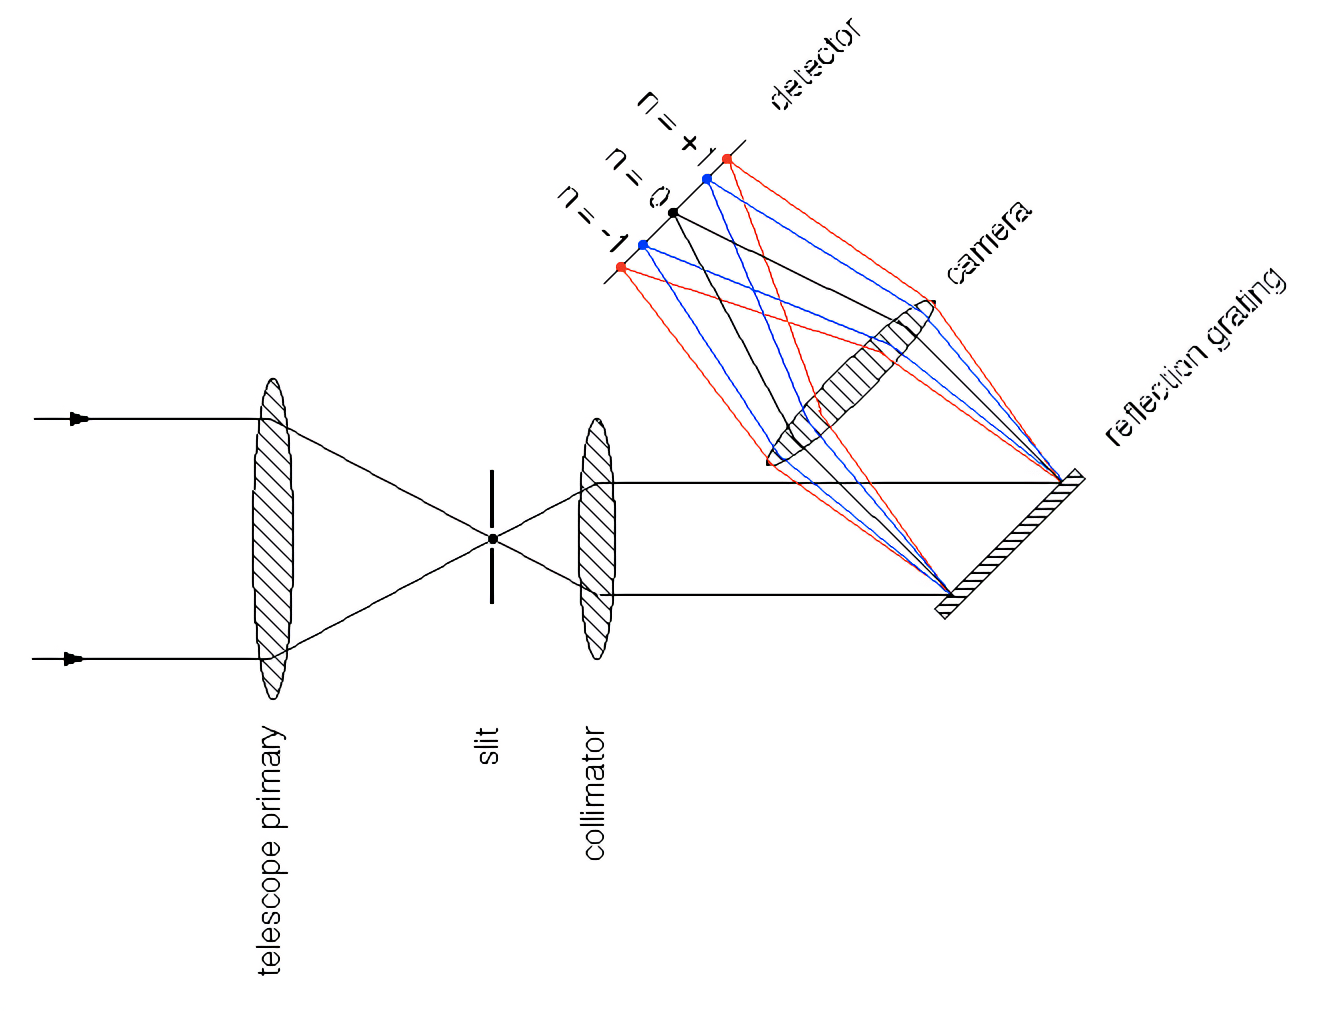
\includegraphics[width=\columnwidth]{spectrograph_refl-transformed.png}
				\captionsetup{font=scriptsize}
				\caption{Diagram of a sample spectrograph setup\cite{vik}. The primary lens focuses the incident light through a slit. The collimator makes the rays parallel as they diffract off of the reflection grating. A last lens focuses the rays on the detector.}
				\label{fig:spectrograph}
			\end{figure}
		
		\subsection{Arc Lamp}
			
		\subsection{Data Reduction}
			When taking measurements with the spectrograph there exists a level of background noise which must be accounted for to ensure accurate measurements. Removing this noise is known as data reduction\cite{manual}. This noise comes from many things including readout electronics, thermal emissions, and non-uniformities in the detector\cite{astropy}.
			
		Diffraction grating and equation + figure, what is the spectrograph setup, arc lamps + emission lines
		flats and biases
	
	\section{Methodology}
		\subsection{Apparatus}
			\begin{figure}
				\includegraphics[width=\columnwidth]{ccdDiagram.png}
				\captionsetup{font=scriptsize}
				\caption{Diagram showing the physical setup of the experiment\cite{manual}. The apparatus follows the diagram in figure \ref{fig:spectrograph} with the addition of a neutral density filter to reduce the intensity of the light at all wavelengths. The focal lengths of the focussing lens, collimator and demagnifying lens were 100mm, 225mm and 50mm respectively.}
				\label{fig:apparatus}
			\end{figure}
		
			The apparatus was setup as shown in figure \ref{fig:apparatus} and all lenses were moved to be approximately at the right position to focus the light. The Atik 314L+ CCD was used for this experiment. The CCD was kept below -5 degrees to negate the effect of thermal noise on the detector.
	
		\subsection{Determining Readnoise and Gain}
			To calibrate the CCD, the readnoise and gain need to be calculated. These quantities are calculated using two flats and two biases as follows in equations \ref{eq:gain} and \ref{eq:readnoise}\cite{manual}.
			
			\begin{equation}
				\text{gain} = \frac{(\overline{\text{flat}_1} + \overline{\text{flat}_2}) - (\overline{\text{bias}_1} + \overline{\text{bias}_1})}{\sigma_{flatdif}^2 - \sigma_{biasdif}^2}
				\label{eq:gain}
			\end{equation}
			\begin{equation}
				\text{readnoise} = \text{gain} \times \frac{\sigma_{biasdif}}{\sqrt{2}}
				\label{eq:readnoise}
			\end{equation} where $\overline{\text{flat}_n}$ are the mean pixel value of the nth flat frame and $\overline{\text{bias}_n}$ the same for the nth bias frame, while $\sigma_{flafdif}$ and $\sigma_{biasdif}$ are the standard deviations of these pixel values. 30 bias frames were taken at an exposure of 0.001 seconds, the lowest possible exposure, and 15 flat frames were taken at 	0.1 seconds. For a pair of bias frames and flat frames, the gain and readnoise were calculated. To increase precision, the calculations for gain and readnoise were repeated for 7 pairs of flats and 15 pairs of biases and then averaged to get average and uncertainty values.
		
		\subsection{Wavelength Calibration}
			To calibrate the spectrograph with respect to wavelength a mercury arc lamp was used. As the wavelength of the emission lines of the mercury lamp were known, see figure \ref{fig:mercury}, these lines could be used to identify the lines in the detection and hence a wavelength could be assigned to each x value of the frame.
			
			\begin{figure}
				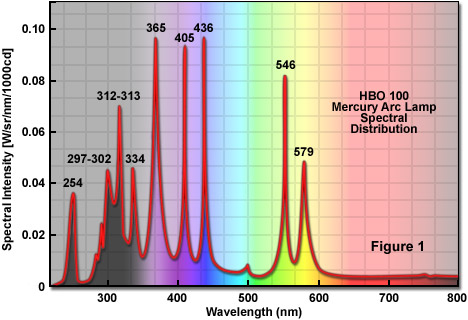
\includegraphics[width=\columnwidth]{mercurySpectrum.jpg}
				\captionsetup{font=scriptsize}
				\caption{The emission spectrum of a mercury arc lamp shown by ZEISS\cite{zeiss}. As the wavelength of each emission line is known, they can be used to calibrate the spectrograph.}
				\label{fig:mercury}
			\end{figure}
			
	
		\subsection{Determining the Resolution of the Spectrograph}
	
	\section{Results and Analysis}
		The gain was calculated to be $(1.58 \pm 0.74)\times 10^{-3}$ and readnoise was calculated to be $(36.5 \pm 17.3) \,\text{electrons}$. The uncertainties on these measurements was taken as the standard deviation of the list of gains and readnoises.
		
	
	\section{Conclusion}
	
	\printbibliography
\end{document}